\chapter{PatchMatch Based Joint View Selection and Depthmap Estimation} \label{ch:patchmatch}

\section{Introduction} 

\begin{figure*}
\centering
    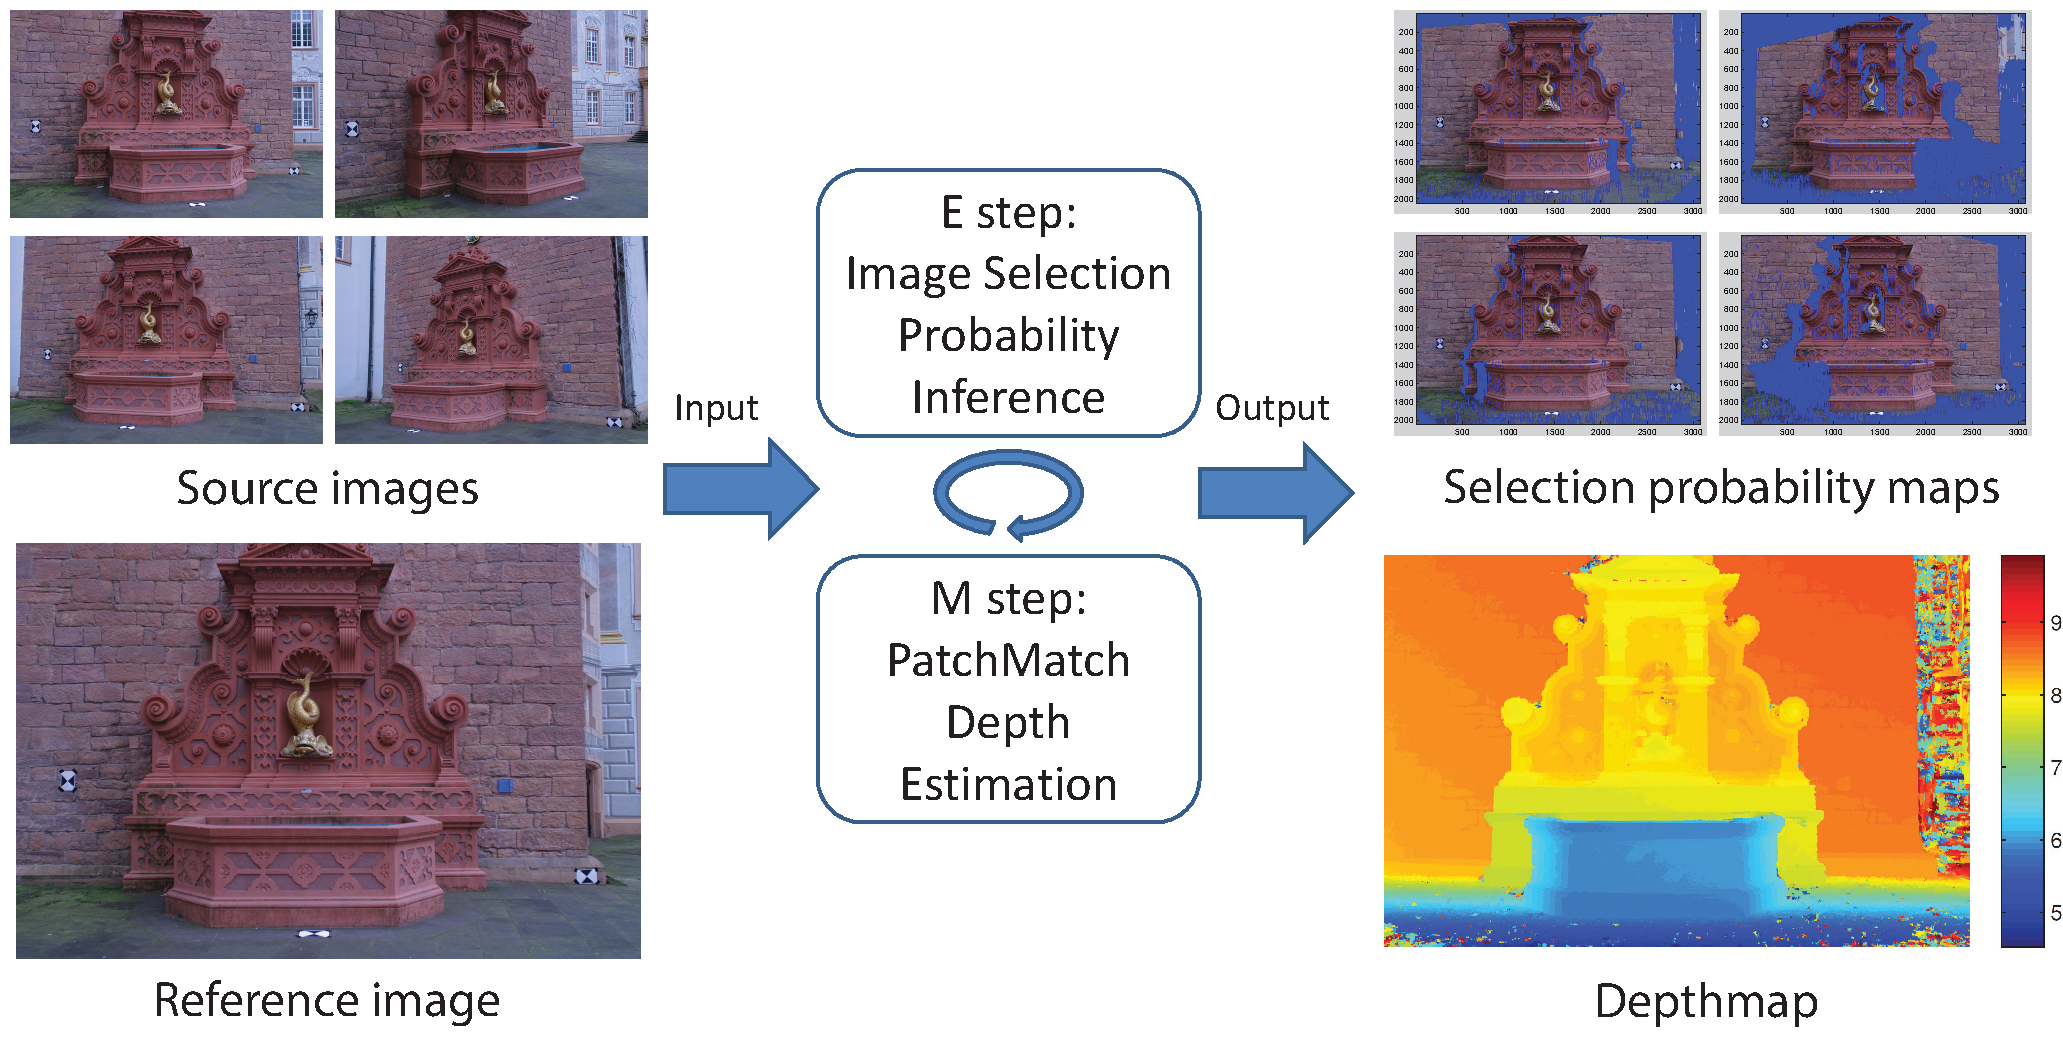
\includegraphics[width=1\columnwidth]{chapter3/resource/combine.pdf}
    \caption[Overview of joint view selection and depthmap estimation.]{Overview of our  approach. Input imagery is used to jointly estimate a depthmap and pixel level view associations. Blue regions in the view selection probability map indicate pixels in the reference image lacking reliable observations in the corresponding source image.}
\label{fig:selectionExample}
\end{figure*}

Multi-view depthmap estimation (MVDE) methods strive to determine a view dependent depthfield by leveraging the local photoconsistency of a set overlapping images observing a common scene.
Applications benefiting from high quality depthmap estimates include dense 3D modeling, classification/recognition \cite{CVPR_kinect} and image based rendering \cite{View_interpolation1993}.
However, achieving highly accurate depthmaps is inherently difficult even for well controlled environments where factors such as viewing geometry, image-set color constancy, and optical distortions are rigorously measured and/or corrected.
Conversely, practical challenges for robust depthmap estimation from non-controlled input imagery (\ie Internet collected data) include mitigating heterogeneous resolution and scene illuminations, unstructured viewing geometry, scene content variability and image registration errors (\ie outliers). Moreover, the increasing availability of  crowd sourced datasets has explicitly brought efficiency and scalability to the forefront of application requirements, while implicitly increasing the importance of data association management when processing such large scale datasets. 

The input for MVDE is commonly assumed to consist of a convergent set of images along with reliable estimates of their pose and calibration parameters. The extracted depthmap will correspond to the pixel-wise 3D structure hypotheses that best explain the available image observations in terms of some measure of visual similarity \wrt  a reference image.
% Namely, pair wise local photoconsistency is a noisy measurement of 3D structural correspondence
Ironically, the potential robustness afforded by having multiple available images is compromised by the inherent variability in pairwise photoconsistency observations. In practice, correct depth hypotheses may provide low photoconsistency in a source image subset (e.g. occlusions or  illumination aberrations), while incorrect depth hypotheses may register high image similarity (e.g. repetitive structure or homogeneous texture). These technical challenges render multi-view depth hypothesis evaluation as a problem of robust model fitting, where a demarcation among inlier and outlier photoconsistency observations is required.
%For controlled capture environment a priori heuristic determination are generally sufficient
We tackle this implicit data association problem by addressing the question: {\em What aggregation subset of the source image set should be used to estimate the depth of a particular pixel in the reference image}.

We propose a probabilistic framework  for depthmap estimation that jointly models pixel-level view selection and depthmap estimation given pairwise image photoconsistency. An overview is depicted in Figure \ref{fig:selectionExample}. The corresponding graphical model is solved by EM-based view selection probability inference and PatchMatch-like depth sampling and propagation. Our approach iteratively alternates between exploration of  the depth search space and updating our formulated probabilistic model. The insight leveraged by our method is the spatial smoothness in the photoconsistency at the correct depth hypothesis of a given pixel \wrt the images in the source image dataset \cite{CombinedDepthOutlier,Goesele07}.
Our expectation of  having a high overlap of photoconsistent source images among neighboring pixels in the reference image, leads to modeling  the depth estimation problem as a Markov process where the unobserved states correspond to binary indicator variables for the selection probability of each source image.

We summarize the contributions and advantages of the framework as follows.
\begin{enumerate}
\item
{\bf Accuracy:} Mitigation of spurious data associations at the pixel level provides state-of-the-art accuracy results for single depthmap estimation.
\item
{\bf Efficiency:} Deployment of PatchMatch sampling and propagation enables reduced computational burden as well as GPU implementation.
\item
{\bf Scalability:} Linear storage requirement \wrt the number of source images, as opposed to the exponential growth in the joint view selection and depth estimation model by \citet{CombinedDepthOutlier}, enables handling selection instances comprising hundreds of images.
\end{enumerate}

\section{Joint View Selection and Depth Estimation} \label{sec:view_selection_stereo}
In this section we provide an overview of our PatchMatch propagation scheme (Section \ref{sec:PatchMatch}), describe our probabilistic graphic model (Section \ref{sec:model}), describe our variational inference approximation to the model's  posterior probability  (Section \ref{sec:variationalInfer} and Section \ref{sec:updateSchedule}) and finalize describing our implementation  (Section \ref{sec:algorithm}).

\subsection{PatchMatch Propagation for Stereo} \label{sec:PatchMatch}

Our algorithm uses single oriented planes instead of the multiple oriented planes \cite{patchMatchParallel},
to reduce the three-dimensional search space (depth and two angles for the orientated plane) to one dimension. We alternatively perform upward/downward propagations during the odd iterations and  perform rightward/leftward propagations during even iterations. To calculate the depth at pixel $(i,j)$ for the rightward propagation, only the depth at positions $(i,j-1)$ and $(i,j)$ are tested on pixel $(i,j)$ (Figure \ref{fig:propagation}). Likewise, only one neighbor is considered for all other propagations. The propagation schemes of \cite{patchMatchStereo1} and \cite{patchMatchParallel} are shown in Figure  \ref{fig:propagation}.

In the absence of proper depth hypotheses, we additionally draw and test $H$ random depth hypotheses for each pixel during propagations. We use $H=1$ and have 3 depth hypotheses tested per pixel in a propagation, i.e. the depths of current and the neighboring pixel along with one random depth. Without loss of generality,  we limit our discussion henceforth to  the rightward horizontal propagation.

\begin{figure}
\centering
%\subfloat{
%    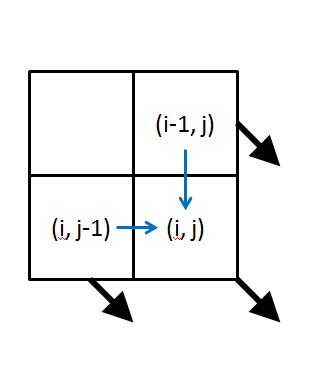
\includegraphics[height=0.34\columnwidth]{chapter3/resource/propagationPatchMatch.png}
%}
%\subfloat{
%    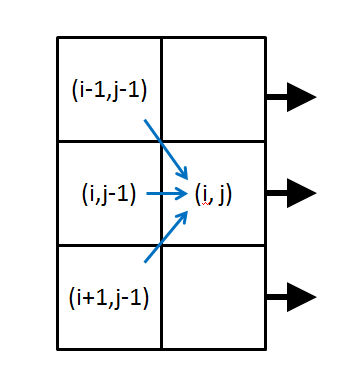
\includegraphics[height=0.34\columnwidth]{chapter3/resource/propagationScaleRobust.png}
%}
%\subfloat{
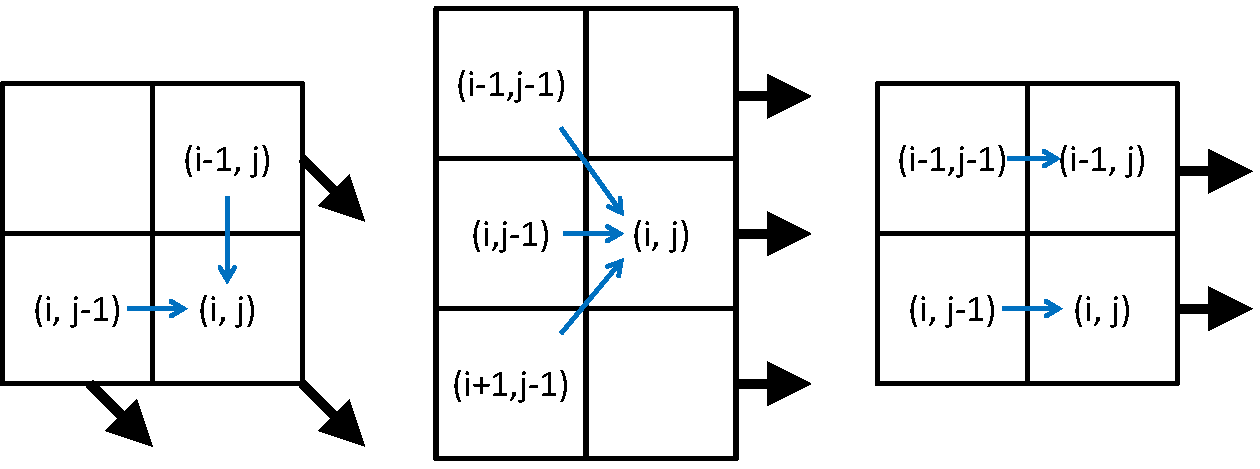
\includegraphics[width=0.99\textwidth]{chapter3/resource/prop_cropped.pdf}
%}
\caption[Illustration of three differernt PatchMatch propagation schemes.]{The black and blue arrows show the propagation directions and the sampling schemes. Left: Top left to bottom right propagation in \cite{patchMatchStereo1}. Middle: Rightward propagations in \cite{patchMatchParallel}. Right: Our rightward propagation.}
\label{fig:propagation}
\end{figure}

\subsection{Graphical Model} \label{sec:model}
In our algorithm, the depth is estimated for a reference image $X^{\text{ref}}$, given a set of $M$ (unstructured) source images $X^1, X^2, ... X^M$ with known camera calibration parameters, which are the output of a typical structure from motion system such as VisualSFM \cite{WuVSFM}. We denote the correct depth associated with each pixel $l$ on image $X^{\text{ref}}$ as $\theta_l$.

Photo-consistency values for the correct depth of a given pixel across a set of source images may be incongruent for some of the source images. This may be attributed to a diversity of factors such as occlusions, calibration errors, illumination aberration, etc.
Therefore, depth estimation for a given pixel entails the determination of which subset of source images will provide the most robust estimate. Our model defines $M$ binary variables $Z_l^m\in{\{0,1\}}, m = 1, 2...M$ for each pixel $l$ in the reference image $X^{\text{ref}}$, where $Z_l^m$ is 1 if image $X^m$ is selected for depth estimation of pixel $l$, and 0 otherwise.

\begin{figure}
\centering
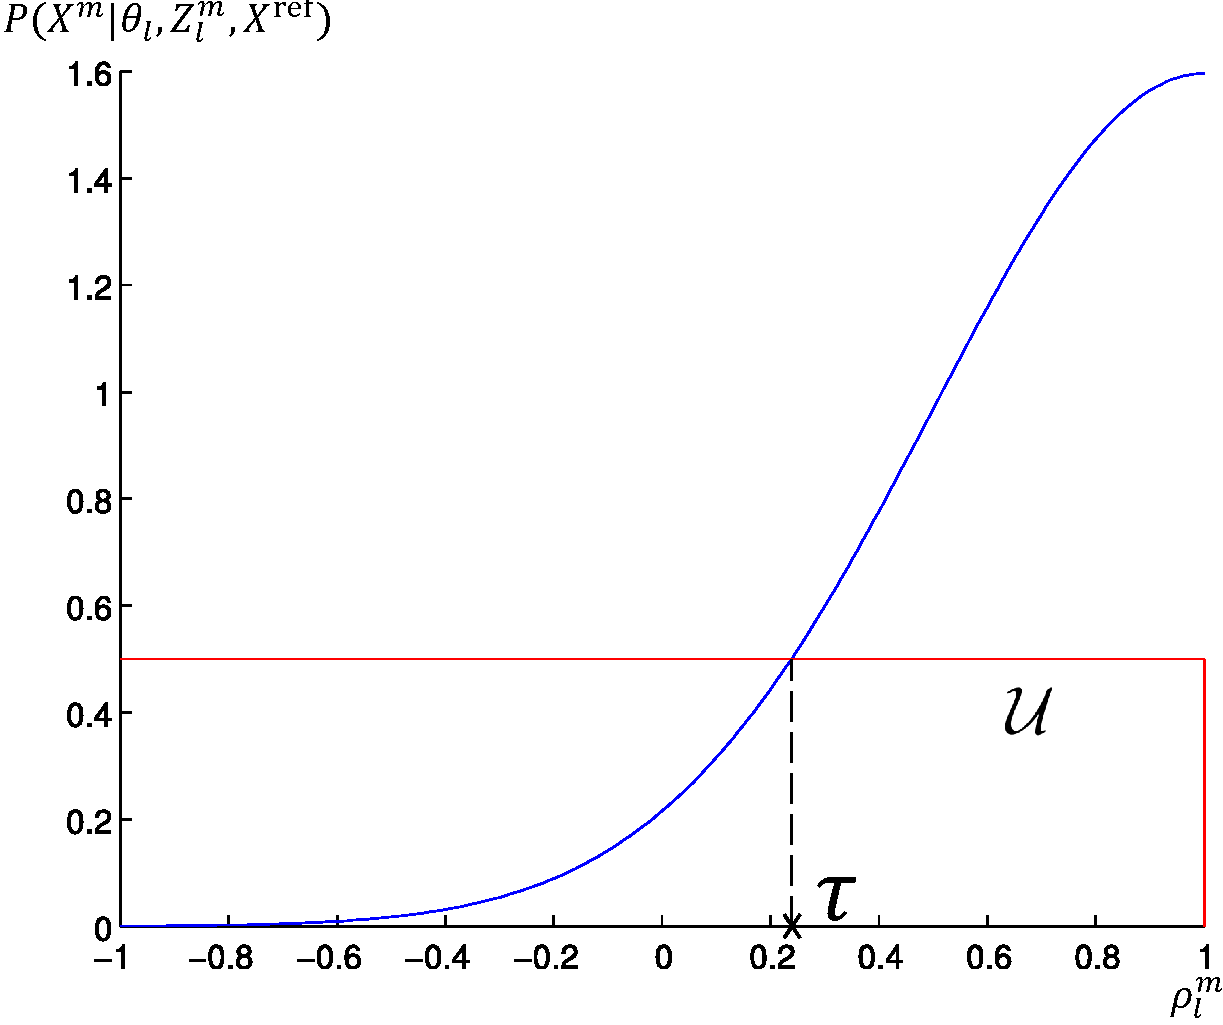
\includegraphics[width=0.6\textwidth]{chapter3/resource/figure_obmodel_cropped.pdf}
\caption[Distribution of the likelihood function.]{Distribution of Equation (\ref{equ:observationModel})}
\label{fig:obModelDistribution}
\end{figure}

We first define the likelihood function. We denote the color patch centered at pixel $l$ in the reference image as $X_l^{\text{ref}}$. Given a pixel $l$ and its correct depth $\theta_l$ in the reference image $X^{\text{ref}}$, a color patch $X_l^m$ on source image $m$ can be determined through homography warping \cite{Shen_TIP2013}. If $Z_l^m=1$, the probability that the observed color patch $X_l^m$ is color-consistent with $X_l^{\text{ref}}$ should be high. We use NCC (normalized cross correlation) to compare the two color patches $X_l^m$ and $X_l^{\text{ref}}$ as a robust proxy to single pixel comparisons, and denote the NCC measurement as $\rho_l^m$. In the case when $Z_l^m=0$, $X_l^m$ has arbitrary colors due to factors such as occlusion or calibration errors, so the probability of observing $X_l^m$ is unrelated to $X_l^{\text{ref}}$ and considered uniformly distributed. Therefore we propose the following likelihood function
\begin{equation}
P(X_l^m|Z_l^m, \theta_l, X_l^{\text{ref}}) \text{=}
\begin{cases}
        \frac{1}{NA}e^{-\frac{(1-\rho_l^m)^2}{2\sigma^2}} & \text{if } Z_l^m\text{= }1\\
       \frac{1}{N} \mathcal{U} & \text{if } Z_l^m\text{= } 0\label{equ:observationModel},
\end{cases}
\end{equation}
where $A$ equals to $\int_{-1}^1exp\{-\frac{(1-\rho)^2}{2\sigma^2}\}d\rho$ and $N$ is a constant. Note that NCC value ranges in $[-1,1]$ and equals 1 with the best color consistency. Consistent with our intuition, a color patch $X_l^m$ with high NCC value $\rho_l^m$ has high probability $P(X_l^m|Z_l^m=1, \theta_l,X_l^{\text{ref}})$. $\mathcal{U}$ is the uniform distribution in the range $[-1,1]$ with probability density 0.5. Note that NCC computation is affine invariant and multiple pairs of color patches can generate the same NCC value. To simplify the analysis without affecting depthmap quality, Equation (\ref{equ:observationModel}) assumes the number of color patches $X_l^m$ that can generate any specific NCC value is the same and equals to $N$. Since only the ratio $P(X_l^m|Z_l^m=1, \theta_l, X_l^{\text{ref}})/P(X_l^m|Z_l^m=0, \theta_l, X_l^{\text{ref}})$ matters in the model inference discussed in Section \ref{sec:variationalInfer} and Section \ref{sec:updateSchedule}, we can safely ignore the constant $N$ in Equation (\ref{equ:observationModel}).


In Equation (\ref{equ:observationModel}) $\sigma$ is the parameter determining the suitability of an image  based on NCC measurement $\rho_l^m$. As seen in Figure \ref{fig:obModelDistribution}, a soft threshold $\tau$  is determined by $\sigma$. If $\rho_l^m$ is larger than $\tau$, it is more likely that image $m$ is selected, and vice versa. Since $X_l^{\text{ref}}$ is observed for each pixel, $P(X_l^m|Z_l^m, \theta_l, X_l^{\text{ref}})$ is simply denoted as $P(X_l^m|Z_l^m, \theta_l)$ in the rest of the paper.


The depths of  nearby pixels are considered independent, while the pairwise smoothness is put on the nearby selection variables along the current propagation direction (Figure \ref{fig:model}) through the transition probabilities:
\begin{equation}
P(Z_l^m|Z_{l-1}^m)= \left( \begin{smallmatrix} \gamma & 1- \gamma \\ 1-\gamma& \gamma \end{smallmatrix} \right).
\label{equ:transitionProb}
\end{equation}
Setting $\gamma$ close to 1 encourages  neighboring  pixels to have similar selection preference for source images $X^m$. To enable parallel computation, we only enforce pairwise constraint on the pixels of the same row in the horizontal propagations. Note Figure  \ref{fig:model} only shows one row of selection variables for each of the source images.

\begin{figure}
\centering
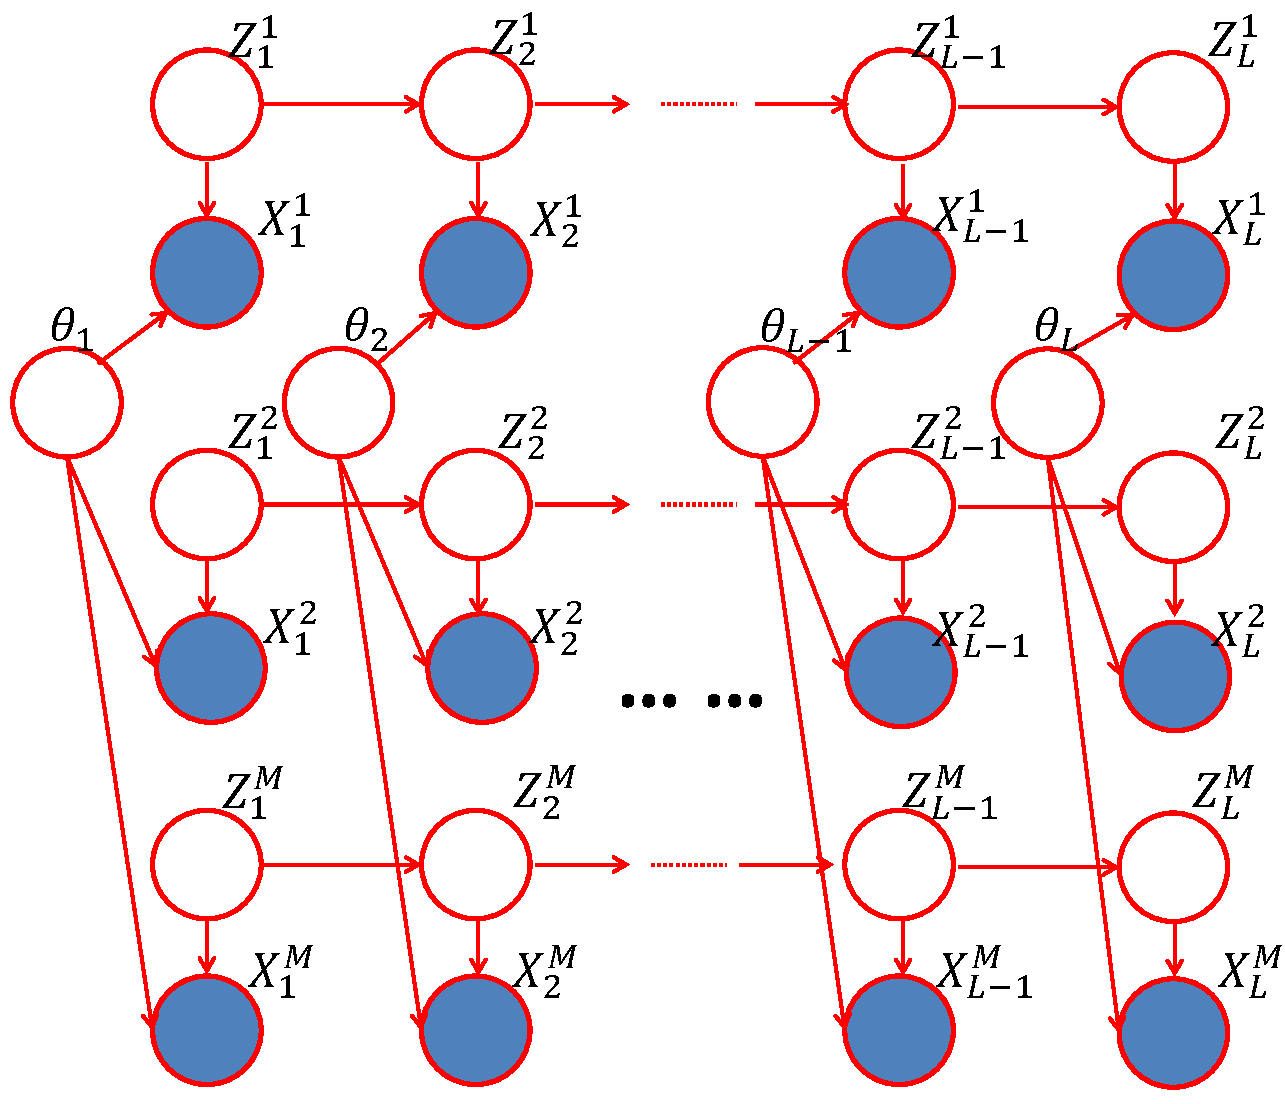
\includegraphics[width=0.7\textwidth]{chapter3/resource/graphicalModel_cropped.pdf}
\caption[Graphical model of joint view selection and depthmap estimation.]{The graphical model. $\theta_l$ is the depth of pixel $l$. $Z_l^m$ is the selection of image $m$ at pixel $l$. $X_l^m$ is the observation (colors) on the source image $m$ given depth $\theta_l$.}
\label{fig:model}
\end{figure}

Finding the optimal selection $\bm{Z}$ and depth $\bm{\theta}$ given all the images $\bm{X}$ equates to computing the maximum of the posterior probability (MAP) $P(\bm{Z}, \bm{\theta}|\bm{X})$. The Bayesian approach firstly computes the joint probability based on the graphical model (Figure \ref{fig:model}) and normalizes over $P(\bm{X})$. The joint probability is
\begin{equation}
P(\bm{X},\bm{\theta},\bm{Z}) = \prod_{m=1}^M{[ P(Z_1^m)} \prod_{l=2}^L{P(Z_l^m|Z_{l-1}^m)}\prod_{l=1}^{L}{P(X_l^m|Z_l^m ,\theta_l)}]\prod_{l=1}^{L}P(\theta_l),
\label{equ:jointProb}
\end{equation}
where $L$ is the number of pixels along the propagation direction of the reference image. We use an uninformative uniform distribution for prior $P(Z_1^m)$ as well as depth prior $P(\theta_l)$ since we have no preference without observations. However, computing $P(\bm{X})$ is intractable as it requires to sum over all possible values of $\bm{Z}$ and $\bm{\theta}$.

We interleave pixel level inference of image selection probability with fixed depth, and depth updating with fixed image selection probability.
Our approach is a variant of the generalized EM (GEM) \cite{Neal98aview}.  Similarly to the work by  \citet{Neal98aview}, we use variational inference theory to justify our algorithm.


%%%%%%%%%%%%%%%%%%%%%%%%%%%%%%%%%%%%%%%%%%%%%%%%%%%%%%%%%%%%%%%%%%%%%%%%%%%%%%%%%%%%%%%%%%%

%%%%%%%%%%%%%%%%%%%%%%%%%%%%%%%%%%%%%%%%%%%%%%%%%%%%%%%%%%%%%%%%%%%%%%%%%%%%%%%%%%%%%%%%%%%

\subsection{Variational Inference} \label{sec:variationalInfer}
Variational inference is to consider a {\em restricted} family of distributions $q(\bm{Z}, \bm{\theta})$ and then seek the member of this family to approximate the real posterior distribution $P(\bm{Z}, \bm{\theta}|\bm{X})$, in the sense that the KL divergence between these two is minimized \cite{BishopBook}. {\em The restriction is imposed purely to achieve tractability.} The real posterior distribution is over the set of unobserved variables $\bm{\theta}=\{\theta_l| l = 1,...,L\}$ and $\bm{Z} = \{\bm{Z}^m| m = 1,...,M\}$, where $\bm{Z}^m = \{Z_1^m, Z_2^m, ..., Z_L^m\}$ is a chain in the graph. We put restrictions on the family of distributions $q(\bm{Z},\bm{\theta})$, assuming that it is factorizable into a set of distributions \cite{BishopBook}:
\begin{equation}
q(\bm{Z},\bm{\theta})  = \prod\nolimits_{m=1}^M{q_m(\bm{Z}^m)}\prod\nolimits_{l=1}^L{q_l(\theta_l)}.
\label{equ:approximateDistribution}
\end{equation}
For tractability, we further constrain each $q_l(\theta_l)$, $l = 1, 2, ... ,L$ to the family of Kronecker delta functions:
\begin{equation}
q_l(\theta_l) = \delta(\theta_l = \theta_l^*) =
\begin{cases}
    1,              & \text{if } \theta_l = \theta_l^{*} \\
    0,              & \text{otherwise}
\end{cases}
\end{equation}
where $\theta_l^{*}$ is a parameter to be estimated. This assumption is in contrast to most other works \cite{Strecha_BayesModelCVPR2004,CombinedDepthOutlier,Sun_ECCV2002_stereoBeliefProp,Sun_CVPR2005_stereo}, which discretize the depth as a means to recover the whole posterior distribution of the depth. Once the distribution $q_l(\theta_l)$ is determined, $\theta_l$ is set to $\theta_l^*$ to maximize the approximate posterior distribution Equation (\ref{equ:approximateDistribution}), so $\theta_l^*$ is actually the final estimated depth. Conversely, the depths $\bm{\theta}$ can be considered as parameters shared by different chains instead of as variables. This assumption seamlessly combines the PatchMatch sampling scheme in the graph model inference.

The variational method seeks to find a member $q^{\text{opt}}(\bm{Z},\bm{\theta}) \text{=} \prod_{m\text{=}1}^M{q_m^{\text{opt}}(\bm{Z}^m)}\prod_{l\text{=}1}^{L}{q_l^{\text{opt}}(\theta_l)}$ from the family  $q(\bm{Z},\bm{\theta})$,  minimizing the KL divergence between $q(\bm{Z},\bm{\theta})$ and $P(\bm{Z}, \bm{\theta}|\bm{X})$ under the constraint that $q_m(Z^m), m=1,...M$ are normalized ($q_l(\theta_l)$ is guaranteed to be normalized as it is constrained to be a Kronecker delta function):
\begin{equation}
\begin{aligned}
& \underset{q(\bm{Z}, \bm{\theta})}{\text{minimize}}
& & \text{KL}(q(\bm{Z}, \bm{\theta})||P(\bm{Z},\bm{\theta}|\bm{X})) \\
& \text{subject to}
& & \sum\nolimits_{Z^m}{q_m(Z^m)=1} \text{, } m = 1, \ldots, M.
\end{aligned}
\label{equ:KLobjective}
\end{equation}
%Next we will show, how the coordinate ascent method, which optimizes over one distribution (either $q_m(\bm{Z}^m)$ or $q_l(\theta_l)$) at a time with other distributions fixed, is applied to find $q^{\text{opt}}(\bm{Z},\bm{\theta})$ that optimizes Eq. (\ref{equ:KLobjective}).
Note the optimization is performed over distributions, but not over variables.
%To optimize over $q_m(\bm{Z}^m)$, we substitute Eq. (\ref{equ:jointProb}) into Eq. (\ref{equ:KLobjective}), and take the functional derivative of the Lagrangian with respective to $q_m$. Then set the derivative to 0 (\cite{Koller+Friedman:09}).
To optimize over $q_m(\bm{Z}^m)$, the standard solution \cite{BishopBook} is $\log{(q_m(\bm{Z}^m))} = \mathbb{E}_{\backslash m}[\log{(P(\bm{X},\bm{\theta},\bm{Z}))}]+const$, where $\mathbb{E}_{\backslash m}$ is the  expectation of $\log{(P(\bm{X},\bm{\theta},\bm{Z}))}$ taken over all variables not in $q_m(\bm{Z}^m)$ \cite{BishopBook}. Then we have
\begin{equation}
{q_m^{\text{opt}}(\bm{Z}^m)}\\
%=\sum_{\bm{\theta}}{q(\bm{\theta})}[ln\{\Psi(\bm{Z}^m)
%\prod_{p=1}^{T}{P(X_l^m|Z_l^m,\theta_l})\}]+c\\
\propto{\Psi(\bm{Z}^m)
\prod\nolimits_{l=1}^{L}{P(X_l^m|Z_l^m,\theta_l=\theta_l^*})},
\label{equ:approximateDistZ}
\end{equation}
where $\Psi(\bm{Z}^m) \text{=} P(Z_1^m)\prod_{l=2}^{l=L}P(Z_l^m|Z_{l-1}^m)$.
%$q_m(\bm{Z}^m)$ is evaluated with $\theta_l^*$, $l=1,2,...,L$ fixed.
The right side of Equation (\ref{equ:approximateDistZ}) has form of joint probability of a Hidden Markov Chain with fixed transition probability from Equation (\ref{equ:transitionProb}) and fixed emission probability Equation (\ref{equ:observationModel}). The probability of each hidden variable $q(Z_l^m)$ can be efficiently inferred by forward-backward algorithm \cite{BishopBook}. %$c$ in Eq. (\ref{equ:approximateDistZ}) is a constant, which cancels off in normalizing $q(Z^m_l)$.
See Section \ref{sec:updateSchedule} for more details. This corresponds to the E step of the GEM algorithm.

To optimize over $q_l(\theta_l)$ we seek an optimal parameter $\theta_l^{\text{opt}}$ for the distribution $q_l(\theta_l)$ that minimizes Equation (\ref{equ:KLobjective}). Suppressing the terms  not involving $\theta_l$ gives
\begin{equation}
\theta_l^{\text{opt}} \text{= }  \underset{\theta_l^*}{\text{argmax}} \sum_{m=1}^{M}{q(Z_l^m \text{=}1)\ln{ P(X_l^m|Z_l^m\text{=}1, \theta_l\text{=}\theta^*_l)}}.
\label{equ:approximateDistTheta}
\end{equation}
By substituting Equation (\ref{equ:observationModel}) into Equation (\ref{equ:approximateDistTheta}), we get
\begin{equation}
\theta^{\text{opt}}_l= \underset{\theta^*_l}{\text{argmin}} \sum\nolimits_{m=1}^{M}{q(Z_l^m=1) (1-\rho_l^m)^2 },
\label{equ:approximateDistTheta2}
\end{equation}
where $\rho_l^m$ is a function of $\theta_l^*$. To find $\theta_l^{\text{opt}}$ in the above equation, 3 depth hypotheses sampled based on PatchMatch are tested, and the one that maximizes Equation (\ref{equ:approximateDistTheta2}) is assigned to the parameter of the distribution $q_l(\theta_l)$. This step is the M step of the GEM algorithm.
Note that the righthand side of Equation (\ref{equ:approximateDistTheta2}) is a weighted sum of $(1-\rho_l^m)^2$ with weight equal to the image selection probability. Hence, a small value of $q(Z_l^m=1)$,  designating image $m$ as not favorable, contributes less in evaluating the parameter $\theta_l^*$. %(the depth on pixel $l$). %This exactly coincides to our intuition.

\textbf{Improvement}: Equation (\ref{equ:approximateDistTheta2}) is computationally expensive for hundreds of source images. Based on Equation (\ref{equ:approximateDistTheta2}), it is unnecessary to compute $\rho_l^m$ if the corresponding image selection probability $q(Z_l^m=1)$ is very small.
%Conversely,  a certain amount of good images are enough to estimate the depth.
Hence, we propose a Monte Carlo  based approximation \cite{BishopBook}. Rewriting Equation (\ref{equ:approximateDistTheta2}) as
\begin{equation}
\theta^{\text{opt}}_l= \underset{\theta^*_l}{\text{argmin}} \sum\nolimits_{m=1}^{M}{ P(m)(1-\rho_l^m)^2 }
\label{equ:approximateDistTheta3}
\end{equation}
where the new distribution $P(m) = \frac{q(Z_l^m=1)}{\sum_{m=1}^M{q(Z_l^m=1)}}$ can be deemed  as the probability of image $m$ being the best for depth estimation of pixel $l$. We draw samples based on the distribution $P(m)$ to obtain a subset $S$, then
\begin{equation}
\theta^{\text{opt}}_l= \underset{\theta^*_l}{\text{argmin}}\frac{1}{|S|}\sum\nolimits_{m\in{ S }}{ (1-\rho_l^m)^2 }.
\label{equ:approximateDistTheta4}
\end{equation}
Empirically, 15 samples  suffice to attain good results.

Both distributions $q_m^{\text{opt}}(\bm{Z})$ and $q_l^{\text{opt}}(\theta_l)$ are coupled.
The computation of $\theta_l^*$ requires $q(Z_l^m)$ to be known (Equation (\ref{equ:approximateDistTheta2})), but to infer $q(Z_l^m)$ in Equation (\ref{equ:approximateDistZ}), we need $\theta_l^*$ available. The next subsection introduces the update scheme that computes the distributions iteratively.


%%%%%%%%%%%%%%%%%%%%%%%%%%%%%%%%%%%%%%%%%%%%%%%%%%%%%%%%%%%%%%%%%%%%%%%%%%%%%%%%%%%%%%%%%%%

%%%%%%%%%%%%%%%%%%%%%%%%%%%%%%%%%%%%%%%%%%%%%%%%%%%%%%%%%%%%%%%%%%%%%%%%%%%%%%%%%%%%%%%%%%%


\subsection{Update Schedule} \label{sec:updateSchedule}
\begin{figure}
\centering
    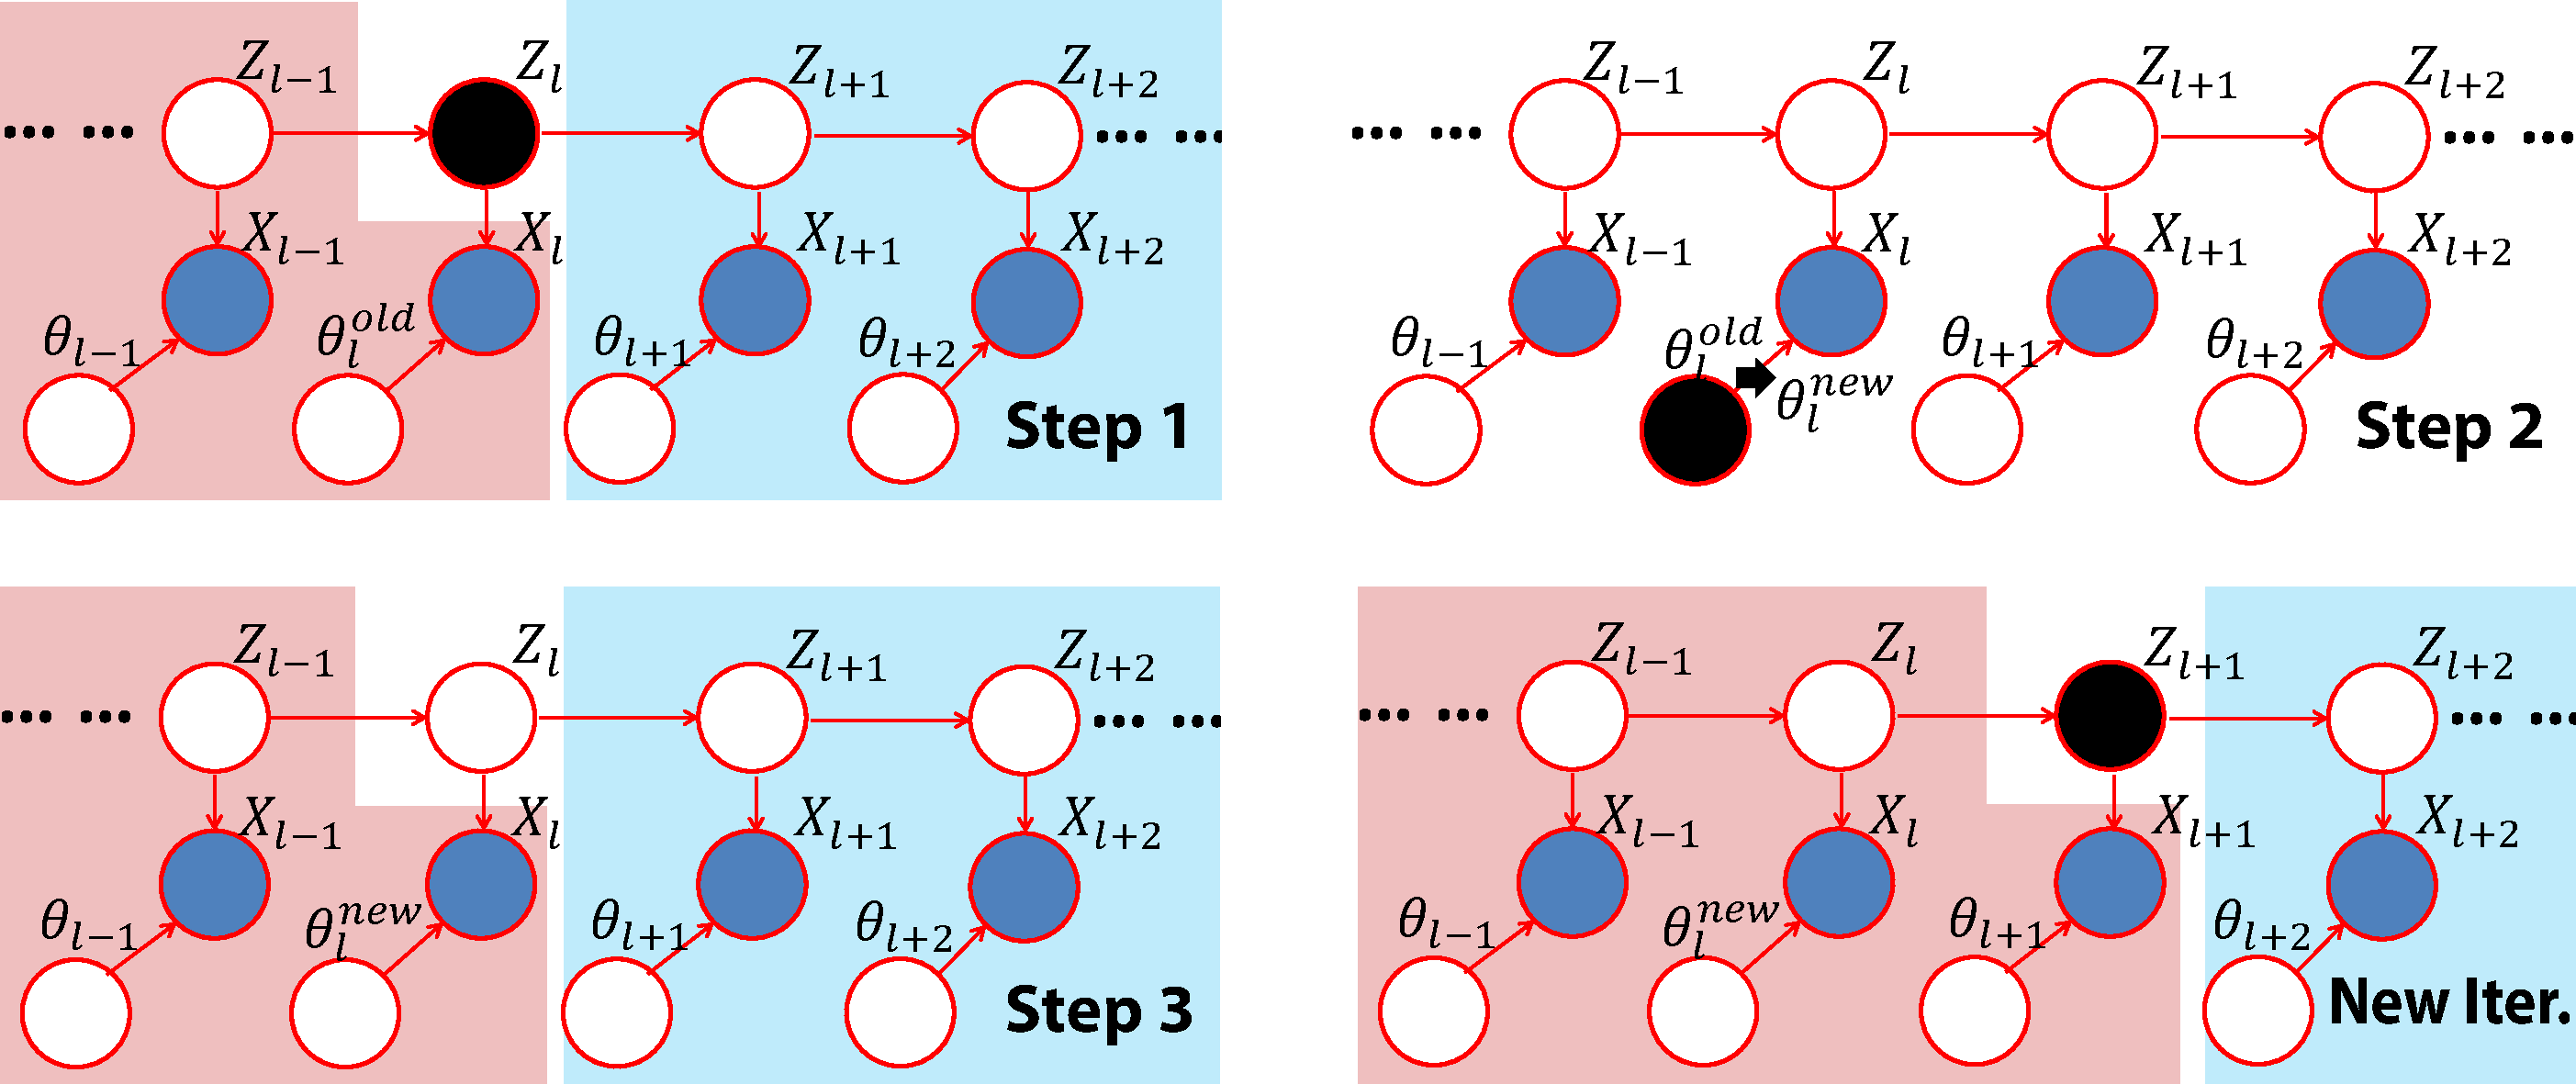
\includegraphics[height=0.42\columnwidth]{chapter3/resource/combine_upschedule.pdf}
\caption[Illustration of the update scheme for the depth and the image selection probability.]{Update schedule. See text for more details.}
\label{fig:updateSchedule}
\end{figure}

The common way to compute approximate distributions is coordinate descent optimization method. Namely, one distribution is optimized while other distributions remain fixed.  Choosing which distribution to optimize over in each step is arbitrary or scheduled based on application, but it always decreases the cost function in Equation (\ref{equ:KLobjective}). %For our multiview stereo depth estimation, we can update all the $q_l(\theta_l)$ first with all $q_m(\bm{Z}^m)$ fixed, and then apply forward-backward algorithm to infer all $q_m(\bm{Z}^m)$ with all $q_l(\theta_l)$ fixed. However
We choose to interleave updates of $q_l(\theta_l)$ and $q_m(\bm{Z}^m)$ as it is able to quickly propagate the correct depth into nearby pixels. For clarity, our explanations below use one chain and omit the image index $m$ for each variable.

For more details on Hidden Markov Chain inference, we refer the reader to text \cite{BishopBook}. The forward-backward algorithm is used to infer the probability of hidden variables $Z_l$.
\begin{equation}
q(Z_l) = \frac{1}{A}\alpha(Z_l)\beta(Z_l),
\label{equ:qZDistribution}
\end{equation}
where A is the normalization factor. $\alpha(Z_l)$ and $\beta(Z_l)$ are the forward and backward message for variable $Z_l$ computed using the following Equations,
\begin{equation}
\alpha(Z_l) = p(X_l|Z_l, \theta_l)\sum_{Z_{l-1}}{\alpha(Z_{l-1})P(Z_l|Z_{l-1})},
\label{equ:forwardMessageUpdate}
\end{equation}
\begin{equation}
\beta(Z_l)=\sum_{Z_{l+1}}\beta(Z_{l+1})P(X_{l+1}|Z_{l+1}, \theta_{l+1})P(Z_{l+1}|Z_{l}).
\label{equ:backwardMessage}
\end{equation}
Both the forward and backward messages are computed recursively (e.g.  $\alpha(Z_l)$ is computed using $\alpha(Z_{l-1})$). In Figure \ref{fig:updateSchedule}, the variables covered in red area and blue area contribute to the forward and backward messages respectively.

We perform the following update schedule as is shown in Figure \ref{fig:updateSchedule}. In step 1, compute $q(Z_l)$ using Equation (\ref{equ:qZDistribution}), (\ref{equ:forwardMessageUpdate}) and (\ref{equ:backwardMessage}) for each source image (\ie $q(Z_l^m)$,$m=1...M$). In step 2, update the depth from $\theta_l^{old}$ to $\theta_l^{new}$ using Equation (\ref{equ:approximateDistTheta2}) or Equation (\ref{equ:approximateDistTheta4}).
%To update depth $\theta_l$, we should compute the selection probability for each of the images, \ie $q(Z_l^m)$,$m=1...M$.
In step 3, with $\theta_l^{new}$, we recompute forward message $\alpha(Z_l)$, which is further used to compute $\alpha(Z_{l+1})$ recursively in Equation (\ref{equ:forwardMessageUpdate}). Next we start at variable $Z_{l+1}$ with the same process until reaching the end of the row in the image. Before the update process, the backward message for each variable can be computed recursively (Equation (\ref{equ:backwardMessage})) and stored in memory.


%%%%%%%%%%%%%%%%%%%%%%%%%%%%%%%%%%%%%%%%%%%%%%%%%%%%%%%%%%%%%%%%%%%%%%%%%%%%%%%%%%%%%%%%%%%
%%%%%%%%%%%%%%%%%%%%%%%%%%%%%%%%%%%%%%%%%%%%%%%%%%%%%%%%%%%%%%%%%%%%%%%%%%%%%%%%%%%%%%%%%%%


\subsection{Algorithm Integration}  \label{sec:algorithm}
%In this subsection, we detail the algorithm given the above formula.
\begin{table}
    \small
    \centering
    \begin{tabular}{|l|c|c|}
        \hline
        \multicolumn{3}{|p{13.0cm}|}{{\bf Input}: All images, depthMap (randomly initialized or from previous propagation)}  \\
        \multicolumn{3}{|p{13.0cm}|}{{\bf Output}: Updated depthMap}\\
        \multicolumn{3}{|p{13.0cm}|}{$m$ -- image index, $l$ -- pixel index}\\
        \hline
            & Eq. & Step \\ \cline{2-3}
            {\bf For} $l = L$ to $1$ & &\\
                \hspace{5 mm} {\bf For} $m = 1$ to $M$  & & \\
                    \hspace{10 mm} Compute backward message $\beta_l^m$  &    (\ref{equ:backwardMessage}) &   1 \\
            {\bf For} $l = 1$ to $L$ & &\\
                \hspace{5 mm} {\bf For} $m = 1$ to $M$ & &\\
                  \hspace{10 mm} Compute forward message $\alpha_l^m$  &      (\ref{equ:forwardMessageUpdate}) & 1\\
                  \hspace{10 mm} Compute $q(Z_l^m)$                    &    (\ref{equ:qZDistribution}) & 1\\
                \hspace{5 mm} Draw depth hypotheses by PatchMatch & &\\
                \hspace{5 mm} Estimate $\theta_l^*$ for $q_l(\theta_l)$ &   (\ref{equ:approximateDistTheta2} or \ref{equ:approximateDistTheta4})& 2\\
                \hspace{5 mm} {\bf For} $m = 1$ to $M$  & &\\
                  \hspace{10 mm} Recompute forward message $\alpha_l^m$ & (\ref{equ:forwardMessageUpdate}) & 3\\
        \hline
    \end{tabular}
\caption[Algorithm of a row/column propagation for joint view selection and depth estimation.]{The algorithm of a row/column propagation.}
\label{table:algorithm}
\end{table}

We now describe the computational framework implementing our  depth estimation and view selection formulation.
The depthmap is initialized with random values within the depth range. Alternatively, sparse 3D measurements may be included within our initialization. Next, the rightward, downward, leftward and upward propagations are applied in sequence. Each propagation (except in the first iteration) uses the depth results of the former propagation. Within each propagation, updates of the depth and the selection probability are interleaved as described in Section \ref{sec:updateSchedule}. After two or three sweeps, each containing the four direction propagations, the depthmap reaches a stable state.  Convergence may alternatively be verified through tracking the number of modified depth estimates up to a threshold. As each row is independent from other rows given our graphical model and processed in exactly the same way during one propagation, it can be easily parallelized for leveraging GPUs. We describe the algorithm for processing one row within rightward propagation in Table \ref{table:algorithm}.



%\subsection{Refinement}
%\section{Discussion}
{\bf Discussion}.
%We discuss some properties of this algorithm in this section.
The estimation of the exact image-wide MAP for our graphical model would require a Hidden Markov Random Field (MRF) formulation instead of our Hidden Markov Chain approximation.
Our choice of using propagation direction specific chain models was driven by computational efficiency/tractability.
The proposed framework enables us to easily interleave the propagation with hidden variable inference while fostering implementation  parallelism.
The enforcement of smoothness constraints on the hidden variables  enables non-oscillating behavior of our evolving depth estimates.
Our PatchMatch based  framework has linear computational and storage complexity \wrt to input data size while being independent of the size of the depth search space.
Namely, since the number of tested depth hypotheses (3 for each propagation) is small and constant, the computation complexity of our method is $O(W H M)$, where $W$, $H$, and $M$ are the width, height and  number of images.  Methods using complete hypotheses search, e.g. \cite{Sun_ECCV2002_stereoBeliefProp, CombinedDepthOutlier}, require  $O(W H M D)$ computations, where D is the size of hypotheses space
%, which is a tradeoff between computation complexity and precision,
normally reaching up to thousands of hypotheses.
 
 
%%%%%%%%%%%%%%%%%%%%%%%%%%%%%%%%%%%%%%%%%%%%%%%%%%%%%%%%%%%%%%%%%%%%%%%%%%%%%%%%%

%%%%%%%%%%%%%%%%%%%%%%%%%%%%%%%%%%%%%%%%%%%%%%%%%%%%%%%%%%%%%%%%%%%%%%%%%%%%%%%%%
\section{Experiments} \label{sec2:experiment}
We evaluate the accuracy of our method on standard ground truth benchmarks and highlight our robustness on multiple crowd sourced datasets.
In both evaluation scenarios we juxtapose our results with current state-of-the-art methods.
We implemented our method in CUDA and executed on a Nvidia GTX-Titan GPU.
For all experiments, the total number multi-directional propagations is set to 3 and we use  $\sigma = 0.45$ in the likelihood function (Equation (\ref{equ:observationModel})) and $\gamma=0.999$ in the transition probabilities (Equation (\ref{equ:transitionProb})).  %refering to Eqs. \ref{equ:observationModel} and  \ref{equ:transitionProb}, respectively.

\begin{table}
\centering
    \begin{tabular}{|c|c|c|c|c|}
    \hline
         &  2cm &  10cm  & 2 cm & 10cm\\
    \hline
    Error & \multicolumn{2}{|c|}{fountain-P11} & \multicolumn{2}{|c|}{Herzjesu-P9}        \\
    \hline
    Ours & 0.732   & 0.911  & 0.619 & 0.833\\
    \hline
    Ours(P)& 0.769   & 0.929  & 0.650 & 0.844\\
    \hline
    LC \cite{LeastCommitment_3DIMPVT2012} & 0.754 &  {0.930} & 0.649 & 0.848 \\
    \hline
    FUR \cite{FURUKAWA_PAMI2010} & 0.731 & 0.838 & 0.646  & 0.836\\
    \hline
    ZAH \cite{Zaharescu_PAMI2011} & 0.712 & 0.832 & 0.220 & 0.501\\
    \hline
    %TYL &0.732 & 0.822 & \textbf{0.658} & 0.852\\
    TYL \cite{TYL} &0.732 & 0.822 & 0.658 & 0.852\\
    \hline
    JAN \cite{JAN} &0.824 & 0.973 & 0.739 & 0.923\\
    \hline
    \end{tabular}
\caption[Percentage of pixels with absolute error less than 2cm and 10cm.]{The percentage of pixels with absolute error less than 2cm and 10cm. Entries {\em Ours(P)}  and {\em Ours}  denote our results with and without postprocessing.  Reported values are from the work by \citet{LeastCommitment_3DIMPVT2012}.}
\label{tab:data}
\end{table}

%%%%%%%%%%%%%%%%%%%%%%%%%%%%%%%%%%%%%%%%%%%%%%%%%%%%%%%%%%%%%%%%%%%%%%%%%%%%%%%%%%%%%%%%%%%%%%%%%%%%%%%%%%%%%%%%%%%%%%%%%%%%%%%%%%%%%%%%%%
%%%%%%%%%%%%%%%%%%%%%%%%%%%%%%%%%%%%%%%%%%%%%%%%%%%%%%%%%%%%%%%%%%%%%%%%%%%%%%%%%%%%%%%%%%%%%%%%%%%%%%%%%%%%%%%%%%%%%%%%%%%%%%%%%%%%%%%%%%%%%%%%%%%%%%%%%%%%%%%%%
%%%%%%%%%%%%%%%%%%%%%%%%%%%%%%%%%%%%%%%%%%%%%%%%%%%%%%%%%%%%%%%%%%%%%%%%%%%%%%%%%%%%%%%%%%%%%%%%%%%%%%%%%%%%%%%%%%%%%%%%%%%%%%%%%%%%%%%%%%

{\bf Ground truth evaluation}. We evaluated on the Strecha datasets (Fountain-P11 and Herzjesu-P9) presented in \citet{Strecha08}  as  they include ground truth 3D structure measurements.
% In contrast to some stereo methods which need manually select the images around the reference view, we input the entire dataset.
We use all dataset images full resolution, set the  NCC patch size to 15 by 15 and  approximate the depth range from sparse 3D points.
 % give the image resolution of 15x15.
We measure pixel-wise depth errors as our goal is to ge\-ne\-rate a single depthmap instead of one consistent 3D scene model.
We calculate the number of pixels with the depth error less than 2cm and 10cm from the ground truth and compare with \cite{LeastCommitment_3DIMPVT2012, FURUKAWA_PAMI2010, Zaharescu_PAMI2011,TYL,JAN}.
All the pixels with accessible ground truth depth are evaluated to convey both the accuracy and the completeness of the estimated depthmaps.
%The ground truth and the depthmaps of the compared methods are obtained by projecting the 3D meshes on each of the reference cameras.
We omit evaluation of the dataset's two extremal views as done by \citet{LeastCommitment_3DIMPVT2012}.
%The same to \cite{LeastCommitment_3DIMPVT2012}, the two extremal views in the datasets are not included in the evaluation.

We use slanted planes of single orientation instead of fronto-parallel planes.
The single dominant orientation direction can be estimated by projecting sparse 3D points onto the ground plane as described in \citet{Gallup07}.
We further apply two optional depthmap refinement schemes to increase the final accuracy.
Our basic depth refinement uses a smaller NCC patch (5x5), while eliminating random depth sampling, during an additional propagation sweep. We then use deterministic fine-grain sampling (20 hypotheses) in the depth neighborhood ($\pm 1$ cm.) of each  pixel's depth estimate as proposed in \citet{Shen_TIP2013}.
Finally, a median filter of size 9x9 is applied  to each raw depthmap. %We denote the results of our method without and with postprocessing as OM1 and OM2.
Table \ref{tab:data} shows our method is comparable to the state-of-the-art methods. Note the results of \citet{LeastCommitment_3DIMPVT2012, TYL, JAN} are obtained through multi-depthmap fusion, while our method directly estimates  individual depthmaps.

\begin{figure}
\centering
\subfloat{
    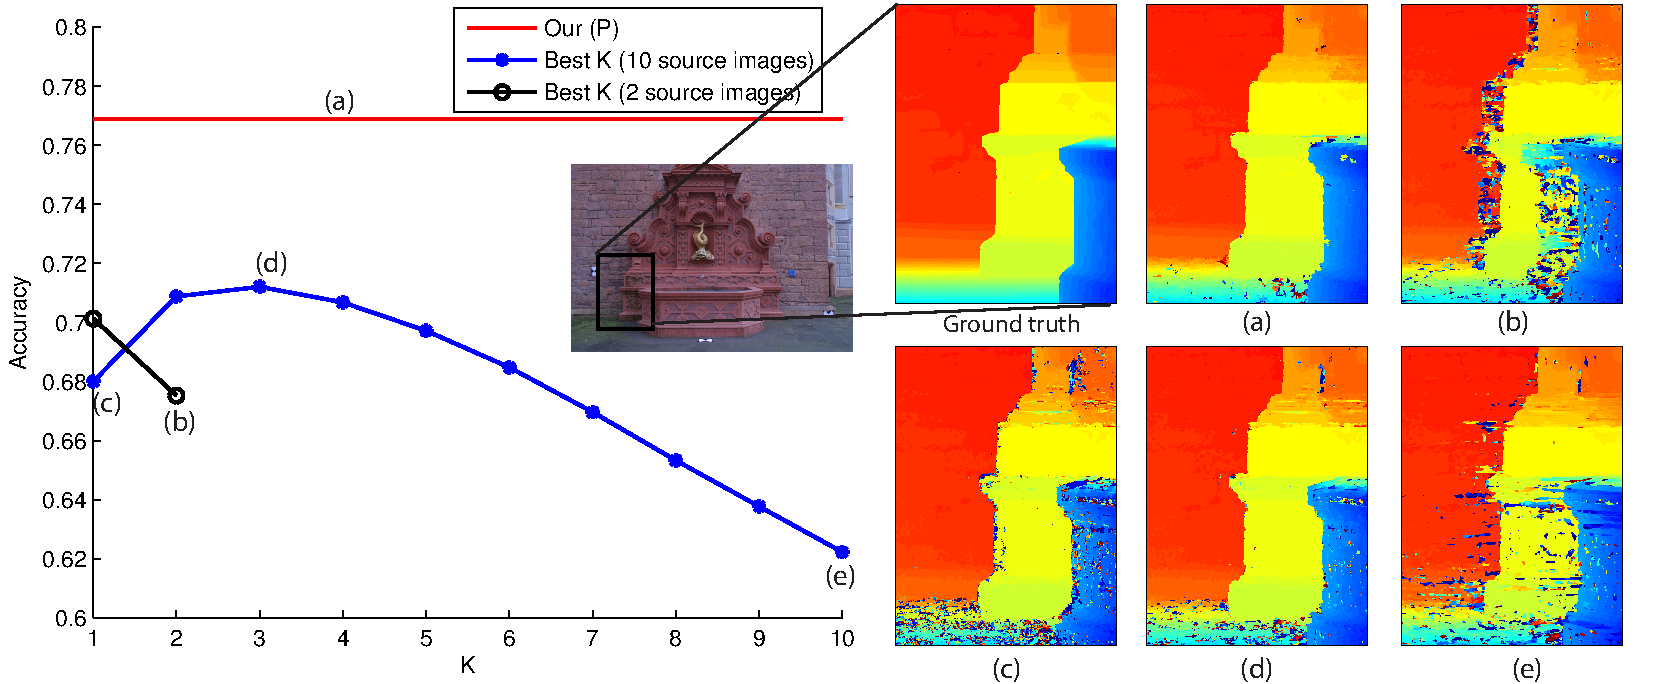
\includegraphics[width=0.96\columnwidth]{chapter3/resource/subregionCombine.pdf}
}
\caption[Comparison against the best-K planesweeping method in accuracy given different $K$.]{Left: Comparison against best-K aggregation. Right: Raw depthmap output of a partially occluded subregion with results for different dataset-aggregation combinations.}
\label{fig:bestK}
\end{figure}

\begin{figure}
\centering
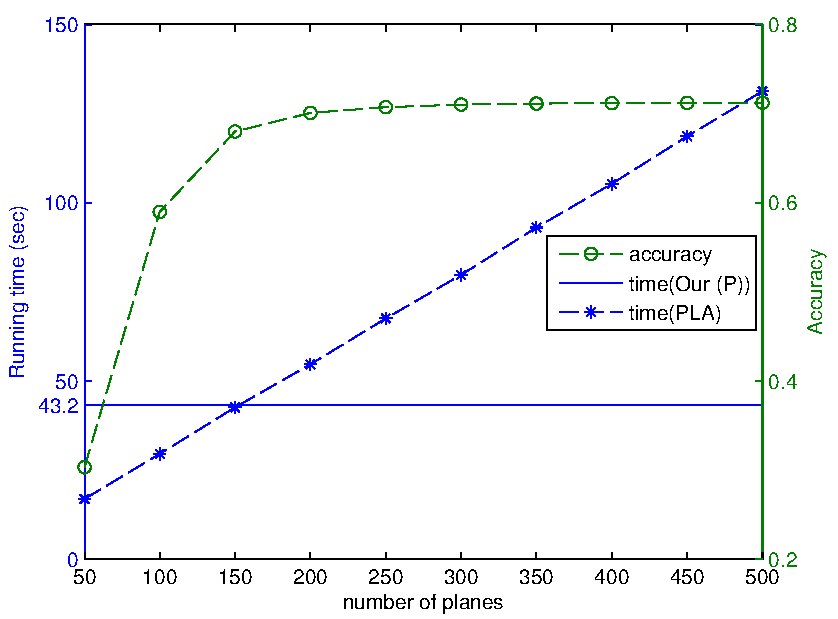
\includegraphics[width=0.7\linewidth]{chapter3/resource/planesweepTiming.pdf}
\caption[Comparison against the best-K planesweeping method in accuracy and run time given different number of planes.]{Fountain dataset performance. Left: Average running time. Right: Percentage of pixels given different thresholds.  PLA is the planesweep algorithm with all source images and K=3, while GOS is the method by \citet{Goesele07}.}
\label{fig:timing}
\end{figure}

{\bf Advantages of pixel level view selection}. Figure \ref{fig:bestK} shows our comparison to the occlusion-robust best-K planesweeping method \cite{handle_occlusion2001}, where
for a given depth hypothesis, the cost is the average of the best K costs, with K being predefined.
When K is set to the number of source images, it degenerates to the basic planesweeping algorithm that computes the cost using all source images.
As opposed to our method with dynamic weights of images used for depth recovery, this method has a worse ability to handle occlusion.
We compute depthmaps of the fountain-P11 data with varying K and otherwise fixed parameters, using 2000 planes.
 %and do the same median filtering afterwards.
The percentage of pixels within 2cm difference from the ground truth is taken as a measure of the error.
We run the planesweeping using two different dataset types. In the first case all 10 source images are used. Alternatively, we use the neighboring left and the right images.
Figure \ref{fig:bestK} shows our results outperform all fixed aggregation schemes and illustrates the raw depthmap output of a partially occluded subregion.



%{\bf Performance and scalability}.
Run times for our method are compared with an optimized GPU planesweeping code.
Figure \ref{fig:timing} shows the linear dependence of computation time to the number of planes as well the diminishing accuracy improvements provided by increasing the search space resolution. Our PatchMatch sampling and propagation scheme only requires depth range specification, foregoing  explicit search space discretization.
 %The number of planes is the tradeoff between depthmap accuracy and computation time.
%As to memory usage, normally the planesweeping needs to store the large cost volume. We conclude that our algorithm beats the planesweeping method in accuracy, speed and memory usage.



{\bf Robustness to noisy SfM estimates}. The  advantage of  pixel-level view selection across the entire dataset is highlighted  in Figure \ref{fig:alexander}, where we compare  our results for corrupted SFM estimates  against those obtained using the approach by \citet{Goesele07}.
%The considered scenario involves a scene with structural symmetry that causes disjoint scene elements  to be incorrectly fused into a single structure.
Figure \ref{fig:alexander} depicts Alexander Nevsky Cathedral in Sofia having indistinguishable structure in the tower structure (\ie view invariant appearance due to structural symmetry). A set of 136 images, comprised by two mutually exclusive subsets observing the front or back, was fed into VisualSFM \cite{WuVSFM} yielding a corrupted 3D model where symmetric structure is fused along with the disjoint camera clusters. The approach by \citet{Goesele07} initially selects a global subset of $~20$ images based  on the corrupted SFM estimates and select  independently for each pixel's depth estimation a fixed number (typically 4) of images from the global subset (similar to using K-best aggregation with K=4). If the global subset is unbalanced or is contaminated by corrupted estimates the completeness of the model is compromised, as shown in Figure \ref{fig:alexander} where the background dome is missing. We consider the entire dataset and implicitly mitigate such outliers. Moreover, we re-executed the code by \citet{Goesele07} with manually filtered camera poses and indeed achieved correct results.

\begin{figure}
\centering
\includegraphics[width=1\linewidth]{chapter3/resource/alexander.pdf}
\caption[Example depthmap output given outlier camera poses.]{\label{fig:alexander} Top: Front and back of Alexander Nevsky Cathedral and estimated 3D model. Bottom: original image, depthmap of our method and the method by \citet{Goesele07} with wrong and correct camera poses.
}
\end{figure}

{\bf Robustness to varying capture characteristics}.
\begin{figure*}
\centering
\includegraphics[width=1\linewidth]{chapter3/resource/allResultsCombine.pdf}
\caption[Example depthmap output on Internet collected photos, and qualitive comparision againt the Goesele's method.]{Each image triplet  depicts a reference image along with our and Goesele's (\cite{Goesele07}) depthmap output (Best viewed in color).}
\label{fig:ipc}
\end{figure*}
We tested our algorithm on  Internet photo collections (IPC)  downloaded from the Flickr  for six different scenes: Paris Triumphal Arch (195 images), Brandenburg Gate (300 images), Notre Dame de Paris (300 images), Great Buddha (212 images), Mt.~Rushmore (206 images) and Berlin Cathedral (500 images). In order to control GPU memory, we optionally resize imagery to no more than 1024 pixels for each dimension. Camera poses were calculated using VisualSFM \cite{WuVSFM}.
 %These images can have large difference in viewpoints, resolutions, and illuminations. Moreover, scene content can vary drastically due to foreground occlusion.
 %Our algorithm handles datasets containing several hundreds of images without any manual image selection.
The average run time for Berlin Cathedral is 98.3 secs/image.
For illustration, sky region pixels are masked out using the method in \citet{skyDetection} as post-processing.
To compare with the method by \citet{Goesele07}, we run the author's code
\footnote{http://www.gris.informatik.tu-darmstadt.de/projects/multiview-environment/}
on the same dataset with default parameters except for setting the matching window size to the same as ours (7x7). The results shown in Figure \ref{fig:ipc} illustrate that, while both approaches are robust to wide variations in illumination, scale and scene occlusions across the  datasets, our approach tends to provide increased completeness of depthmap estimates. We attribute this to our more flexible view selection framework.  In contrast to the method by \citet{Goesele07}, we avoid making initial hard image discriminations through an initial global image subset.

To quantitatively compare the accuracy of our results with the work by \citet{Goesele07}, in the absence of ground truth geometry for crowd source datasets, we revisit the accuracy of both methods in the Strecha Fountain dataset. The method by \citet{Goesele07} rejects outlier depth estimates based on the NCC values and the viewing angles. Hence, we only compare the accuracy of the reliable pixels as classified by \citet{Goesele07} (comprising  75.4\% of total image pixels).  Figure \ref{fig:compareGoesele} shows our approach outperforming both the method in \citet{Goesele07} and planesweep for high accuracy thresholds. We expect the same accuracy ranking to carry over to the crowd sourced data results.



\begin{figure}
\centering
\centering
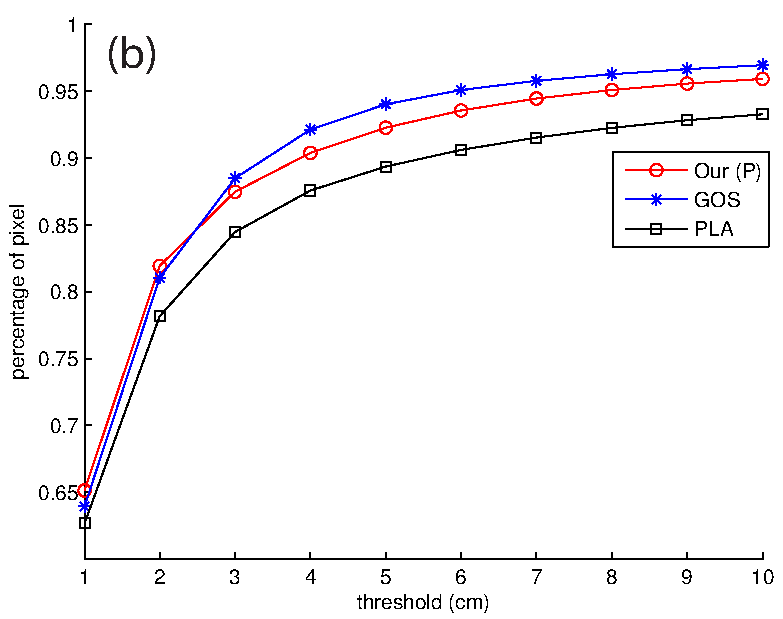
\includegraphics[width=0.60\linewidth]{chapter3/resource/compareGoesele.pdf}
\caption[Comparison again the Goesele's method and the best-K planesweeping method on the fountain dataset.]{Fountain dataset performance.Percentage of pixels given different thresholds.  PLA is the planesweep algorithm with all source images and K=3, while GOS is the method by \citet{Goesele07}.}
\label{fig:compareGoesele}
\end{figure}

%%%%%%%%%%%%%%%%%%%%%%%%%%%%%%%%%%%%%%%%%%%%%%%%%%%%%%%%%%%%%%%%%%%%%%%%%%%%%%%%%%%%

%%%%%%%%%%%%%%%%%%%%%%%%%%%%%%%%%%%%%%%%%%%%%%%%%%%%%%%%%%%%%%%%%%%%%%%%%%%%%%%%%%%%
\section{Conclusion}
We have presented an efficient and effective joint solution to the view selection and depth estimation problem in multi-view stereo. Our solution relies on estimating a selection probability of each source image at the pixel level. The selection probability encodes the existence of contingency issues such as occlusions, specular aberrations and calibration errors. Moreover, by automatically determining reference image data associations with respect to a general source image dataset, we can encompass a larger range input imagery while increasing overall system robustness. Our approach has also extended the PatchMatch algorithm to encompass robust multi-view depth estimation within a probabilistic framework. Reported results achieve state-of-the-art accuracy in ground truth benchmarking while enabling robust operation in crowd-sourced datasets. 

%Future research direction include integrating online normal estimation into our approach in order to reduce the reliance on existing sparse data to initialize our plane sweeping direction. We will explore the use of more sophisticated filtering mechanisms as the ones presented in \cite{Hosni12} in order to improve both computational efficiency and estimation accuracy.

%We presented an efficient and effective method for joint view selection and depthmap estimation. Future research direction includes integrating online plane normal estimation for each pixel. We will explore the use of more sophisticated filtering mechanisms such as the one presented in \cite{Hosni12} to further improve both efficiency and accuracy.



%Note more images used does not mean better depthmap accuracy, and it is useful to remove some unrelated images based on camera poses.
%Here we use the entire dataset to show the scalability and robustness of our algorithm.
%Also we found for very few images, using sparse 3D points from SFM to initialize the depthmap helps the algorithm avoiding false local minima.


%For the Strecha's data, we resize the image to 768X512. The NCC patch size is set to 9X9. It takes around 2.5 seconds to generate one depthmap from 10 source images on NVIDIA Geforce 680. For the internet collected data, generating one depthmap of resolutoin 1024X768 from 289 source images with NCC patch size equal to 9X9 takes around 3 minutes. The memory usage is $O(M*W*H)$, where $M$, $W$, $H$ are the number of images, image width, and image height respectively. The memory is mainly used to store images, NCC cost of the current depth, and the backward messages (Eq. (\ref{equ:backwardMessage})). The memory amount can be largely reduced in trade of more computations by recomputing the cost and backward message in each propagation.

%Using more images does not increase the computation time linearly. The computation relies on several factors. If most target images are not useful to recover the depth, then the number of images used for recover the depth for certain pixel will be significantly smaller than $N$. In this case the computation will be smaller, as some images will never be used to test depth of certain pixels. The computation of $S$ scales linearly with the number of images used.

%\begin{figure} 
%\centering
%    \includegraphics[height=0.6\columnwidth]{resource/bestK/bestK_error.pdf}
%    \caption{The comparison of our method with best K method. }
%\label{fig:bestK}
%\end{figure}

%\begin{table}[t]
%\centering
%    \begin{tabular}{|p{1.3cm}|p{1.7cm}|p{0.95cm}|p{1.2cm}|p{1.2cm}|}
%    \hline
%        Triumphal Arch &  Brandenburg Gate & Notre Dame& Cathedral & Reichstag\\
%    \hline
%        195 & 290 &  290   & 290 &  290\\
%    \hline
%    \end{tabular}
%\label{table:dataSize}
%\caption{The size of each Internet photo collection datasets}
%\end{table}


